\section{Hungarian Grand prix}

\subsection{Circuit Analysis}

\textbf{Circuit Name:} Hungaroring (Mogyoród, Hungary) \\
\textbf{Length:} 4.381 km - \textbf{Laps:} 70 - \textbf{Total Distance:} 306.630 km

\begin{figure}[H]
    \centering
    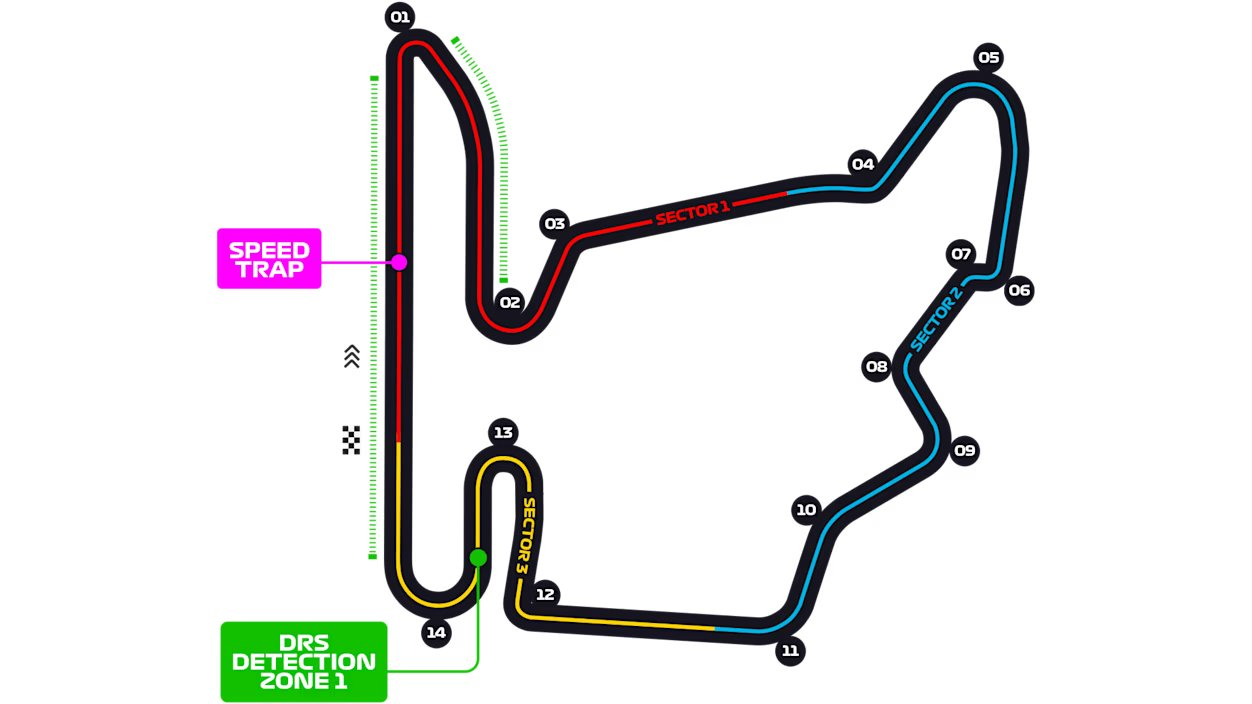
\includegraphics[width=0.75\linewidth]{images/13.Hungary_Circuit.jpg}
\end{figure}


\begin{itemize}
    \item \textbf{Lap Record} : 1:13.447 (2020, Lewis Hamilton – Mercedes).
    
    \item \textbf{Number of Corners \& Key Features} : 14 turns (8 right, 6 left). \\
    Tight and twisty layout, often compared to a "Monaco without walls". High downforce required, limited straights.
    
    \item \textbf{Braking Zones \& Traction} : Heavy braking into Turn 1 (prime overtaking spot) and Turn 12. \\
    Good traction needed out of slow corners to maximise lap time.

    \item \textbf{DRS \& Overtaking} : Two DRS zones (main straight, between Turns 1–2). \\
    Overtaking is difficult due to narrow track and dirty air effect.
    
    \item \textbf{Tyre Degradation \& Strategy} : Circuit demands high downforce and consistent tyre management. \\
    Two-stop strategies typical due to heat and high corner load. 
    
    \item \textbf{Weather \& Environment} : Hot Hungarian summers push tyre temperatures to extremes. \\
    Dusty track surface early in the weekend increases evolution.
\end{itemize}

\textbf{Strategic Summary :}
Hungaroring rewards cars with strong downforce and drivers with precision. Track position is crucial, as overtaking is rare. Heat and tyre wear often decide strategy, making two-stoppers the norm.


\subsection{Race Analysis}

\textbf{Date:} 21 July 2024 — 15:00 local time 

\begin{itemize}
    \item \textbf{Qualifying Summary} : \textbf{Pole Position:} Lando Norris (McLaren) – 1:15.227. \\
    Grid: Piastri 2nd, Verstappen 3rd, Sainz 4th.
    
    \item \textbf{Race Summary} : \textbf{Winner:} Oscar Piastri (McLaren) - his first F1 victory.\\
    \textbf{Podium:} 1. Piastri - 2. Norris - 3. Hamilton.\\
    \textbf{Technical issues:} Gasly (hydraulic problem).\\
    Piastri jumped Norris at start, controlled pace. Hamilton undercut to beat Ferrari. Verstappen struggled with balance, finishing only P5.
    
    \item \textbf{Strategies} : Most front-runners on two-stop strategies (Medium–Hard–Medium). \\
    - McLaren: Piastri gained track position at Turn 1 start, stayed ahead all race. Norris lost time at slow pit stop, finishing P2. \\ 
    - Mercedes: Hamilton on Medium–Hard–Medium. Extended middle stint to overcut Ferrari, securing podium. Russell (17th → 8th + fastest lap) maximised recovery with aggressive undercuts. \\
    - Ferrari: Leclerc on Medium–Hard–Medium, steady pace for P4. Sainz ran Medium–Medium–Hard but lost time late due to tyre wear, P6. \\
    - Red Bull: Verstappen struggled with rear grip, ran Medium–Hard–Hard, unable to challenge podium, P5. Pérez recovered from P16 to P7 on offset Medium–Hard–Medium.
    
    \item \textbf{Performance Trends} : \textbf{McLaren} dominant — car suited Hungaroring perfectly. \\
    Mercedes competitive in race pace. \\
    Ferrari stable but lacking podium pace. \\
    Red Bull off-form — Verstappen complained of poor traction and balance. \\
    Aston Martin and Racing Bulls scrapping for lower points, Haas faded.
    
    \item \textbf{Championship Impact} : \textbf{Drivers:} Verstappen 265 points, Norris 189, Leclerc 162.\\
    \textbf{Constructors:} Red Bull 389, McLaren 338 (+1), Ferrari 322 (-1), Mercedes 241.    
\end{itemize}

\textbf{Key Takeaway :}
McLaren dominated Hungary, with Piastri claiming his first F1 win and Norris close behind. Mercedes showed strong pace, while Red Bull and Ferrari lagged, shifting the competitive balance in the title race.


\subsection{Link \& Takeaway}

\begin{itemize}
    \item Hungaroring’s high-downforce, twisty layout exposed Red Bull’s weaknesses and amplified McLaren’s strengths. 
    \item Piastri’s flawless race execution secured a breakthrough victory, marking him as a genuine contender. 
    \item Norris reinforced McLaren’s strength but lost out via pit stop delay. 
    \item Hamilton’s podium underlined Mercedes’ progress, Russell’s comeback + fastest lap highlighted pace recovery. 
    \item Ferrari maintained consistency but couldn’t match McLaren/Mercedes. 
    \item Aston Martin, Haas, Alpine, and Williams again struggled for points in a tight midfield.
\end{itemize}